\documentclass[12pt]{beamer}
\usepackage[utf8x]{inputenc}
\usepackage{amsmath}
\usepackage{graphics}
\title{Stofftransport \& Reaktionsgleichungen}
\subtitle{Projekt zur Vorlesung Numerische Simulation WS16/17}
\author{P.~Buchfink\inst{1} \and E.~Ott\inst{1} \and M.~Schleicher\inst{1}}
\usetheme{Berkeley}
\usecolortheme{crane}
\institute
{
  \inst{1}
  Institut \\
  Universität Stuttgart
}
\subject{Simulation Technology}

\begin{document}

  \begin{frame}
    \titlepage
  \end{frame}

  \section{RKD-Gleichungen}
    \begin{frame}
      \frametitle{Reaktions-Konvektions-Diffusions-Gleichung}
      $$\frac{\partial C}{\partial t} = \nabla \cdot (D \nabla C) - \nabla \cdot (\vec{v} C) + R(C,t)$$
      {\tiny (\emph{Stochastic Problems in Physics and Astronomy}, Page 41, S. Chandrasekhar, 1943, Reviews of Modern Physics, American Physical Society)}
    \end{frame}

    \begin{frame}
      \frametitle{Zeitschrittbeschränkung}
      Für Diffusion:
      $$\Delta t \leq \frac{\Delta x^2 \Delta y^2}{2D(\Delta x^2 + \Delta y^2)}$$
      {\tiny (\emph{http://pauli.uni-muenster.de/tp/fileadmin/lehre/NumMethoden/WS0910/ScriptPDE/Heat.pdf}, Page 12)}
      
      Für Konvektion: "Vererbt" von Beschränkung für Strömungslöser
    \end{frame}

  \section{Reaktions-gleichungen}
    \begin{frame}
    \frametitle{Lotka-Volterra-Modell}
    $R(C,t)$ nicht analytisch bestimmbar. Modelliert als System von ODEs.
    
    $$\frac{dX_i}{dt} = \alpha_i X_i + \sum_{j=1}^{n} \beta_{ij} X_j$$
    
    Zudem: $\beta_{ii} = -\frac{\alpha_i}{L}$ mit L als Wachstumsgrenze
    \end{frame}
    
    \begin{frame}
    \frametitle{Verhalten \& Stabilität}
    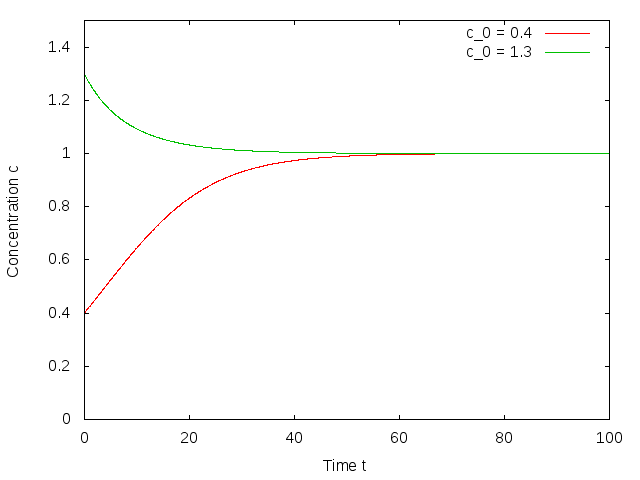
\includegraphics[scale=0.5]{n1_anfangsbedingungen.png}
    \end{frame}
    
    \begin{frame}
    \frametitle{Verhalten \& Stabilität}
    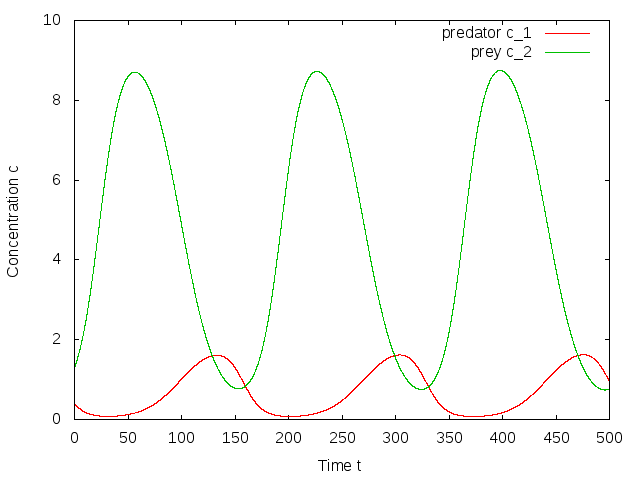
\includegraphics[scale=0.5]{n2_unged_schwingungen.png}
    \end{frame}
    
    \begin{frame}
    \frametitle{Verhalten \& Stabilität}
    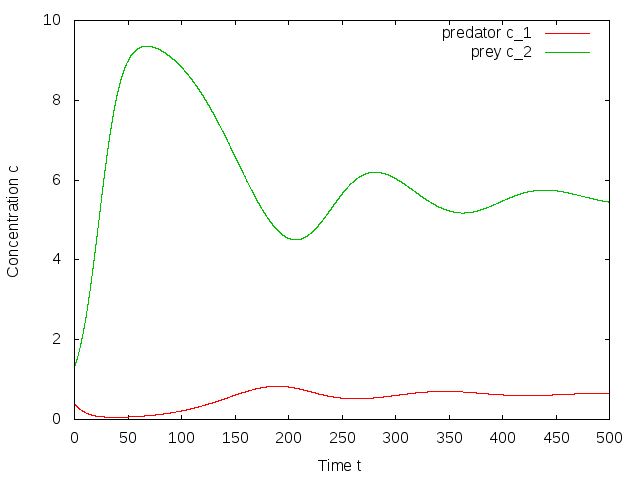
\includegraphics[scale=0.5]{n2_ged_schwingungen.png}
    \end{frame}
    
    \begin{frame}
    \frametitle{Verhalten \& Stabilität}
    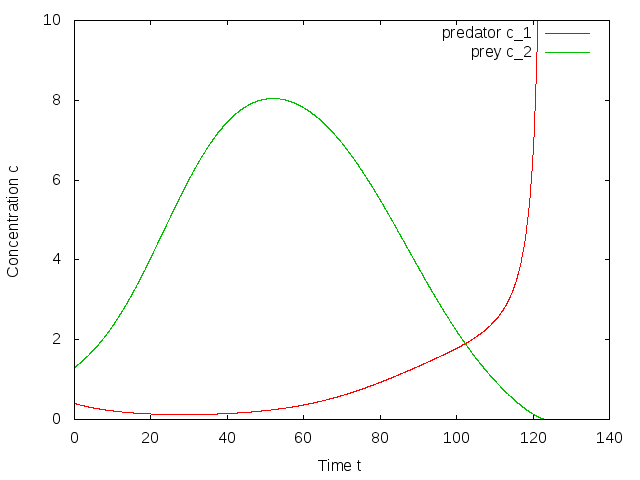
\includegraphics[scale=0.5]{n2_explodiert.png}
    \end{frame}
    
    \begin{frame}
    \frametitle{Verhalten \& Stabilität}
    \begin{itemize}
      \item Instabilität durch Parameter und Löser überlagert
      \item Löser lässt sich durch symplektische Verfahren ersetzen
      \item Parameterwahl nicht trivial, aber auch nicht willkürlich
    \end{itemize}
    \end{frame}
    
    \section{Algenwachstum Szenarien}
    

\end{document}
